\documentclass[letterpaper, 10 pt, conference]{ieeeconf}  % Comment this line out if you need a4paper

%\documentclass[a4paper, 10pt, conference]{ieeeconf}      % Use this line for a4 paper

\IEEEoverridecommandlockouts                              % This command is only needed if 
                                                          % you want to use the \thanks command

\overrideIEEEmargins                                      % Needed to meet printer requirements.

% See the \addtolength command later in the file to balance the column lengths
% on the last page of the document

\usepackage{times}
\usepackage{cite}
\usepackage{graphics} % for pdf, bitmapped graphics files
\usepackage{graphicx}
\usepackage{epsfig} % for postscript graphics files
\usepackage{mathptmx} % assumes new font selection scheme installed
%\usepackage{times} % assumes new font selection scheme installed
\usepackage{amsmath} % assumes amsmath package installed
\usepackage{amsfonts}
\usepackage{amssymb}  % assumes amsmath package installed
\usepackage{bm}
\usepackage{soul}
% \usepackage{todonotes}
\usepackage{url}
\usepackage{multicol}
\usepackage{multirow}
\usepackage[bookmarks=true]{hyperref}
\usepackage{verbatim}
\usepackage{color}
\usepackage{tabularx}
\usepackage{booktabs}
\usepackage{listings}
\usepackage{siunitx}
\usepackage[utf8]{inputenc}
\usepackage{pifont}
\usepackage{csquotes}
\usepackage{mathtools}
\usepackage{breqn}
\usepackage{cancel}
\usepackage{xcolor}
\usepackage{optidef}
\usepackage{cleveref}
\usepackage{setspace}

\usepackage{atbegshi} % to hook to shipout
\usepackage{picture} % for the picture environment

% Copyright (C) 2023  Andrea Patrizi (AndrePatri, andreapatrizi1b6e6@gmail.com)
% 
% This file is part of PhDBiorobBeamerTemplate and distributed under the General Public License version 2 license.
% 
% PhDBiorobBeamerTemplate is free software: you can redistribute it and/or modify
% it under the terms of the GNU General Public License as published by
% the Free Software Foundation, either version 2 of the License, or
% (at your option) any later version.
% 
% PhDBiorobBeamerTemplate is distributed in the hope that it will be useful,
% but WITHOUT ANY WARRANTY; without even the implied warranty of
% MERCHANTABILITY or FITNESS FOR A PARTICULAR PURPOSE.  See the
% GNU General Public License for more details.
% 
% You should have received a copy of the GNU General Public License
% along with PhDBiorobBeamerTemplate.  If not, see <http://www.gnu.org/licenses/>.
% 

% colors
\definecolor{blocktitleviolet}{RGB}{90,123,167}
\definecolor{blockbkgrey}{RGB}{245,245,245}
\definecolor{blockbkgreen}{RGB}{69,163,110}
\definecolor{blockbklightred}{RGB}{255,102,102}
\definecolor{blockbklightblue}{RGB}{111,187,211}

\definecolor{boxbkdarkgrey}{RGB}{160,160,160}
\definecolor{boxbkyellow}{RGB}{206, 209, 177}
\definecolor{boxbkseablue}{RGB}{46, 165, 168}
\definecolor{hhcmblue}{RGB}{16, 114, 175}
\definecolor{boxbklightlighttorquoise}{RGB}{196, 189, 242}
\definecolor{boxbklightlightred}{RGB}{249, 183, 200}

% Define a new command for a larger font size
\newcommand\HUGE{\fontsize{65}{70}\selectfont}

% utilities
% cmd for full citations
\newlength{\mylength} % define a new length \mylength
\newcommand{\fullcitelist}[3][1em]{%
	\setlength{\mylength}{\leftmargin+#1} % set \mylength to \leftmargin + #1
	\begin{enumerate}[label={[#2.\arabic*]}, labelsep=1em, leftmargin=\mylength]
		\forcsvlist{\item \fullcite}{#3}
	\end{enumerate}%
}

% Define a new command named \custombox
% #1: alignment
% #2: width of the box
% #3: color
% #4: text to be displayed inside the box
\newcommand{\custombox}[4]{
	\begin{tcolorbox}[width=#2, colback=#3, colframe=black, left=2pt, right=2pt, top=2pt, bottom=2pt,halign=#1, valign=center]
		#4
	\end{tcolorbox}
}

\ExplSyntaxOn

\seq_new:N \g_contactslist_seq

\NewDocumentCommand{\setCurriculumName}{m}
{
	\tl_gset:Nn \g_curriculum_tl {#1}
}

\NewDocumentCommand{\setFootlineLogo}{m}
{
	\tl_gset:Nn \g_footline_logo_tl {#1}
}

\NewDocumentCommand{\setLocation}{m}
{
	\tl_gset:Nn \g_location_tl {#1}
}

\NewDocumentCommand{\setPosterName}{m}
{
	\tl_gset:Nn \g_proj_tl {#1}
}

\NewDocumentCommand{\setAuthors}{m}
{
	\tl_gset:Nn \g_authors_tl {#1}
}

\NewDocumentCommand{\setCycle}{m}
{
	\tl_gset:Nn \g_cycle_tl {#1}
}

\NewDocumentCommand{\setYear}{m}
{
	\tl_gset:Nn \g_year_tl {#1}
}

\NewDocumentCommand{\setContacts}{m}
{
	\seq_gset_from_clist:Nn \g_contactslist_seq {#1}
}

\NewDocumentCommand{\setUrls}{m}
{
	\seq_gset_from_clist:Nn \g_urllist_seq {#1}
}

\NewDocumentCommand{\getCurriculumName}{}{\tl_use:N \g_curriculum_tl}

\NewDocumentCommand{\getFootlineLogo}{}{\tl_use:N \g_footline_logo_tl}

\NewDocumentCommand{\getLocationName}{}{\tl_use:N \g_location_tl}

\NewDocumentCommand{\getPosterName}{}{\tl_use:N \g_proj_tl}

\NewDocumentCommand{\getAuthors}{}{\tl_use:N \g_authors_tl}

\NewDocumentCommand{\getCycle}{}
{
	\tl_use:N \g_cycle_tl
}

\NewDocumentCommand{\getYear}{}
{
	\tl_use:N \g_year_tl
}

\NewDocumentCommand{\getContactsList}{}
{
	\seq_use:Nn \g_contactslist_seq {;~}
}

\NewDocumentCommand{\getUrlList}{}
{
	\seq_use:Nn \g_urllist_seq {\\}
}

\NewDocumentCommand{\checksetup}{}
{
	\seq_if_empty:NT \g_tutorlist_seq
	{
		\msg_error:nn {PhdBiorobReportTemplate} {no-tutors-set}
	}
	\seq_if_empty:NT \g_contactslist_seq
	{
		\msg_error:nn {PhdBiorobReportTemplate} {no-contacts-set}
	}
	\seq_if_empty:NT \g_urlslist_seq
	{
		\msg_error:nn {PhdBiorobReportTemplate} {no-urls-set}
	}
	\tl_if_empty:NT \g_student_tl
	{
		\msg_error:nn {PhdBiorobReportTemplate} {no-student-set}
	}
	\tl_if_empty:NT \g_proj_tl
	{
		\msg_error:nn {PhdBiorobReportTemplate} {no-projectname-set}
	}
	\tl_if_empty:NT \g_curriculum_tl
	{
		\msg_error:nn {PhdBiorobReportTemplate} {no-curriculum-set}
	}
	\tl_if_empty:NT \g_cycle_tl
	{
		\msg_error:nn {PhdBiorobReportTemplate} {no-cycle-set}
	}
	\tl_if_empty:NT \g_year_tl
	{
		\msg_error:nn {PhdBiorobReportTemplate} {no-year-set}
	}
}

\msg_new:nnn {PhdBiorobReportTemplate} {no-contacts-set} {No~contacts~set!~Please~use~\space\string\setContacts\space.}

\msg_new:nnn {PhdBiorobReportTemplate} {no-urls-set} {No~urls~set!~Please~use~\space\string\setUrls\space.}

\msg_new:nnn {PhdBiorobReportTemplate} {no-curriculum-set} { No~curriculum~has~been~set!~Please~use~\string\setCurriculumName.}

\msg_new:nnn {PhdBiorobReportTemplate} {no-cycle-set} { No~PhD~cycle~has~been~set!~Please~use~\space\string\setCycle.}

\msg_new:nnn {PhdBiorobReportTemplate} {no-year-set} { No~academic~year~has~been~set!~Please~use~\space\string\setYear.}

\NewDocumentCommand{\addPersonalData}{}
{
	\begin{flushleft}
		\vspace{1.5cm}
		\large{\textbf{Student:~}}\large{{\getAuthors}}\vspace{0.2cm}\\
		\large{\textbf{Cycle:~}}\large{\getCycle}\vspace{0.2cm}\\
		\large{\textbf{Tutor(s):~}}\large{{\getTutorsList}}\vspace{0.2cm}\\
		\large{\textbf{Year:~}}\large{\getYear}\vspace{0.2cm}\\
		\large{\textbf{Contacts:~}}\large{\getContactsList}
	\end{flushleft}
}

\NewDocumentCommand{\addResearchProjTitle}{}
{
	\begin{center}
		\textbf{\normalsize{\getProjName}}
	\end{center}
}

\NewDocumentCommand{\addTopLogos}{}
{
	\begin{figure}[t]
		\centering
		\includegraphics[width=0.99\textwidth]{logos/top_logos.pdf}
	\end{figure}
	\hphantom{h}\vspace{1.3cm}
}

\NewDocumentCommand{\addTitlePage}{}
{
	\addTopLogos
	
	\begin{center}
		
		\LARGE{\textbf{Doctorate~in~Bioengineering~and~Robotics }\vspace{0.4cm}\\
			Curriculum:~\getCurriculumName}
		
	\end{center}
	
	\addPersonalData % adds personal data to frontpage
	
	\clearpage
}

\ExplSyntaxOff

\makeatletter

\newlength{\myroundradius}
\setlength{\myroundradius}{5mm} % Default value

\newcommand{\setroundradius}[1]{%
	\setlength{\myroundradius}{#1}%
}

\newcommand{\contentframecolor}{white} % Default content frame color
\newcommand{\setcontentframecolor}[1]{%
	\renewcommand{\contentframecolor}{#1}%
}

\newenvironment{customblock}[5][0pt]{%
	% #1: Optional border thickness (default 0pt)
	% #2: Block title
	% #3: Title Background color
	% #4: Title text color
	% #5: Content Background color
	\begin{tcolorbox}[colback=#3,colframe=#3,arc=\myroundradius,auto outer arc,
		coltext=#4,boxrule=0pt,boxsep=0pt,
		left=5pt,right=5pt,top=\titlepaddingtop,bottom=\titlepaddingbottom]
		\centering\LARGE #2
	\end{tcolorbox}
	\vspace{\titlecontentspace} % Space between title and content
	
	\begin{tcolorbox}[colback=#5,colframe=\contentframecolor,arc=\myroundradius,auto outer arc,
		boxrule=#1,boxsep=5pt,
		left=5pt,right=5pt,top=5pt,bottom=5pt]
	}{
	\end{tcolorbox}
	\vspace{\baselineskip} % Space after the block
}

\newenvironment{customblocknotitle}[2][0pt]{%
	% #1: Optional border thickness (default 0pt)
	% #2: Content Background color
	\begin{tcolorbox}[colback=#2,colframe=\contentframecolor,arc=\myroundradius,auto outer arc,
		boxrule=#1,boxsep=5pt,
		left=5pt,right=5pt,top=5pt,bottom=5pt]
	}{
	\end{tcolorbox}
	\vspace{\baselineskip} % Space after the block
}

\newlength{\titlecontentspace}
\setlength{\titlecontentspace}{0.5cm} % Default value

\newcommand{\settitlecontentspace}[1]{%
	\setlength{\titlecontentspace}{#1}%
}

\newlength{\titlepaddingtop}
\setlength{\titlepaddingtop}{5pt} % Default value for padding above the title

\newlength{\titlepaddingbottom}
\setlength{\titlepaddingbottom}{5pt} % Default value for padding below the title

\newcommand{\settitlepaddingtop}[1]{%
	\setlength{\titlepaddingtop}{#1}%
}

\newcommand{\settitlepaddingbottom}[1]{%
	\setlength{\titlepaddingbottom}{#1}%
}

\NewDocumentCommand{\headline}{ > {\SplitList{,}} m }{%
	% Extract the two paths from the list
	\ProcessList{#1}{\assignlogo}
	\setlogos
}

\newcommand{\assignlogo}[1]{%
	\ifx\firstlogo\@undefined
	\newcommand{\firstlogo}{#1}
	\else
	\newcommand{\secondlogo}{#1}
	\fi
}

\newcommand{\setlogos}{%
	\begin{columns}[b]
		\begin{column}[c]{.85\textwidth}
			\begin{center}
				\begin{HUGE}
					\textcolor{black}{\textbf{\getPosterName}}\\
				\end{HUGE}
			\end{center}
		\end{column}
	\end{columns}
	
	\begin{columns}[b]
		\begin{column}[c]{.3\textwidth}
			\ifx\firstlogo\@empty
			\hbox{} % Empty box if no first logo
			\else
			\hspace{4.0cm}
			\includegraphics[scale=1.4]{\firstlogo}
			\fi
		\end{column}
		\begin{column}[c]{.4\textwidth}
			\begin{center}
				\begin{huge}
					\getAuthors\\
				\end{huge}\vskip1cm
			\end{center}
		\end{column}
		\begin{column}[c]{.3\textwidth}
			\ifx\secondlogo\@empty
			\hbox{} % Empty box if no second logo
			\else
			\hspace{-0.8cm}
			\includegraphics[scale=1.4]{\secondlogo}
			\fi
		\end{column}    
	\end{columns}
	
	\vskip2cm
	
}

\newcommand{\themarker}{$\triangleright$} % Default marker
\newcommand{\settheitemmarker}[1]{%
	\renewcommand{\themarker}{#1}%
}

\makeatother

\linespread{0.98}
\setlength{\textfloatsep}{1pt}  % Replace X with the desired length in points
\setlength{\intextsep}{1pt}
\setlength{\abovecaptionskip}{1pt}


% ### uncomment to produce preprint IEEE copyright notice ###
%\AtBeginShipout{%
%  \AtBeginShipoutUpperLeft{%
%    \put(\dimexpr.5\paperwidth-9cm\relax,-1cm){%
%      \parbox{\textwidth}{\centering\footnotesize%
%        © 2023 IEEE. Personal use of this material is permitted. Permission from IEEE must be obtained for all other uses, in any current or future media, including reprinting/republishing this material for advertising or promotional purposes, creating new collective works, for resale or redistribution to servers or lists, or reuse of any copyrighted component of this work in other works.}%
%    }%
%  }%
%}

\begin{document}
	
\title{\LARGE \bf
A Software Ecosystem for Research in Reinforcement Leaning-based Receding Horizon Control
}

\author{
  \authorblockN{%
    Andrea Patrizi\authorrefmark{1}\authorrefmark{2}, Carlo Rizzardo\authorrefmark{1}, 
    and Nikos G. Tsagarakis\authorrefmark{1}
  }
}

\maketitle

\begingroup\renewcommand\thefootnote{\authorrefmark{2}}
	\footnotetext{Department of Informatics, Bioengineering, Robotics and Systems Engineering, Università di Genova, Via All'Opera Pia 13, 16145 Genova.}
\endgroup

\begingroup\renewcommand\thefootnote{\authorrefmark{1}}
	\footnotetext{Humanoids and Human-Centred Mechatronics (HHCM), Istituto Italiano di Tecnologia (IIT), Via San Quirico 19d, 16163 Genova.}
\endgroup

\setlength{\textfloatsep}{12.0pt plus 8.0pt minus .0pt}

\begin{abstract}
Robotics research in locomotion is undergoing a transformative shift towards the use of learning-based tools. Learning methodologies have been shown to be capable of remarkable robustness and performance even when applied to real-world environments; however, they present limitations in interpretability, safety guarantees and sample efficiency. For this reason, it is the authors' belief that more classical control approaches should not be disregarded yet. We thus advocate for a hybrid approach, combining offline data-based policy design through Reinforcement Learning (RL), with classical online Motion Planning, via Receding Horizon Control (RHC). Even though this kind of hybrid approaches are not entirely new, to the authors' knowledge, there is no specific tool currently available for research in this domain. To this purpose, we developed a modular software ecosystem, hereby briefly presented in its main components and features. 
%We care to stress that the framework is currently under active development, and features might not be stable or could be lacking. 
To facilitate its usability and diffusion, we made all the core components open source under the GPLv2 license. Furthermore, to showcase the potential of our framework and approach, we briefly present a proof-of-concept example combining a high-level RL agent coupled with a lower-level MPC controller for the execution of a simple locomotion task on a simulated quadruped robot.
\end{abstract}

\IEEEpeerreviewmaketitle

\section{A Brief Hystorical Overview: \textnormal{\textit{from Markov Decision Processes and Dynamic Programming to modern Receding Horizon Control and Reinforcement Learning}}}
\begin{figure*}[t]
	\centering
	\vspace{0.1cm}
	\includegraphics[width=0.9\textwidth]{imgs/learning_based_rhc.pdf}
	\caption{Our take on Learning-based Receding Horizon Control: a RHC controller is hierarchically coupled with a higher-level RL agent during both training and real-world deployment. The RL agent has control over key RHC run-time parameters like contact phases and twist commands and can monitor its internal state (costs, constraint violations). The agent learns to exploit the underlying RHC controller to perform the tracking of user-specified high-level task references.}
	\label{fig:lrhc_arch}
\end{figure*}
State-of-the-art of locomotion and manipulation pipelines have been shown to be capable of remarkable performance and robustness~\cite{rl:schneider2023learning,rl:miki2024learning,web::atlas_grip_boston_dyn,web::lrhc_boston_dyn}. These results stand on the shoulders of more than seventy years of research in robotics, control and learning, starting from the very first industrial automated robot \textit{Unimate} in the 1950s~\cite{origins:xu2018fourth}, Richard Bellman's pioneering work in the late 1950s and early 1960s on \textbf{Markov Decision Processes} (MDPs)~\cite{rl:bellman1957markovian} and \textbf{Dynamic Programming}~\cite{rl:bellman1960dynamic} (DP) and the birth of \textbf{Artificial Intelligence} (AI) as an established field of study thanks to the contributions of researchers like Alan Turing, John McCarthy, Marvin Minsky and Claude Shannon.
Specifically, the introduction of the so-called \textit{Bellman equation}~\cite{rl:bellman1960dynamic} for the \textit{Value Function} in conjunction with the formulation of MDPs, laid the foundations of DP as a systematic method for solving sequential decision-making problems by breaking them down into simpler sub-problems~\cite{rl:bellman1960dynamic}. Later on, the development of \textit{Policy Iteration}~\cite{rl:howard1960dynamic}, \textit{TD-learning}~\cite{rl:barto1983neuronlike}, \textit{Q-learning}~\cite{rl:watkins1989learning}, the increased popularization of back-propagation~\cite{rl:rumelhart1986learning} as a way of training powerful neural function approximators and the ever-increasing computational resources progressively paved the way to the ancestors of today's most successful and employed on-policy and off-policy Reinforcement Learning (RL) algorithms PPO~\cite{rl:schulman2017proximal} and SAC~\cite{rl:haarnoja2018soft}, respectively. Some of these ancestors include, for instance, the \textit{Natural Policy Gradient}~\cite{rl:kakade2001natural}, \textit{Deep Q-Networks} (DQN)~\cite{rl:mnih2015human},~\textit{Deep Deterministic Policy Gradient} (DDPG)~\cite{rl:lillicrap2015continuous} and \textit{Trust Region Policy Optimization}~\cite{rl:schulman2015trust} algorithms.
In an analogous way, DP principles served as a foundational basis for the evolution of modern RHC~\cite{modern_mpc:grandia2023perceptive}.
Just as DP breaks down complex problems into smaller subproblems and iteratively finds optimal solutions by considering future consequences, RHC iteratively solves finite-horizon optimal control problems over shorter time intervals, considering system dynamics and constraints. Over the years, many algorithms for the solution of the classical receding-horizon nonlinear optimization problem have been developed, and several of them are directly tied to the continuous-time dynamics evolution of DP, namely \textit{Differential Dynamic Programming} (DDP)~\cite{rhc:jacobson1970differential,rhc:todorov2005generalized,rhc:diehl2009efficient,rhc:tassa2012synthesis}.
%\section{RL versus RHC: \textnormal{\textit{formulation}}}
%\section{RL vs RHC: \textnormal{\textit{shortcomings and advantages}}}

\section{A hybrid approach: \textnormal{\textit{Learning-Based Receding Horizon Control with RL}}}
\begin{figure*}[t]
	\centering
	\vspace{0.1cm}
	\includegraphics[width=0.98\textwidth]{imgs/learning_based_rhc.pdf}
	\caption{Our take on Learning-based Receding Horizon Control: a MPC controller is exposed to a RL agent through key runtime parameters, like contact phases, its internal state (costs, constrains..) and interfaces for setting task commands. The agent learns to exploit the underlying RHC controller to perform the tracking of user-specified high-level task references. This allows to both tackle problems which are non-trivial at the MPC level (like phase selection), while also exploiting the flexibility of the agent to complete tasks and the capability of the MPC of ensuring safety.}
	\label{fig:lrhc_arch}
\end{figure*}
\section{Implementation: \textnormal{\textit{available tools, framework overview and rationale}}}
\begin{figure}[t]
	\centering
	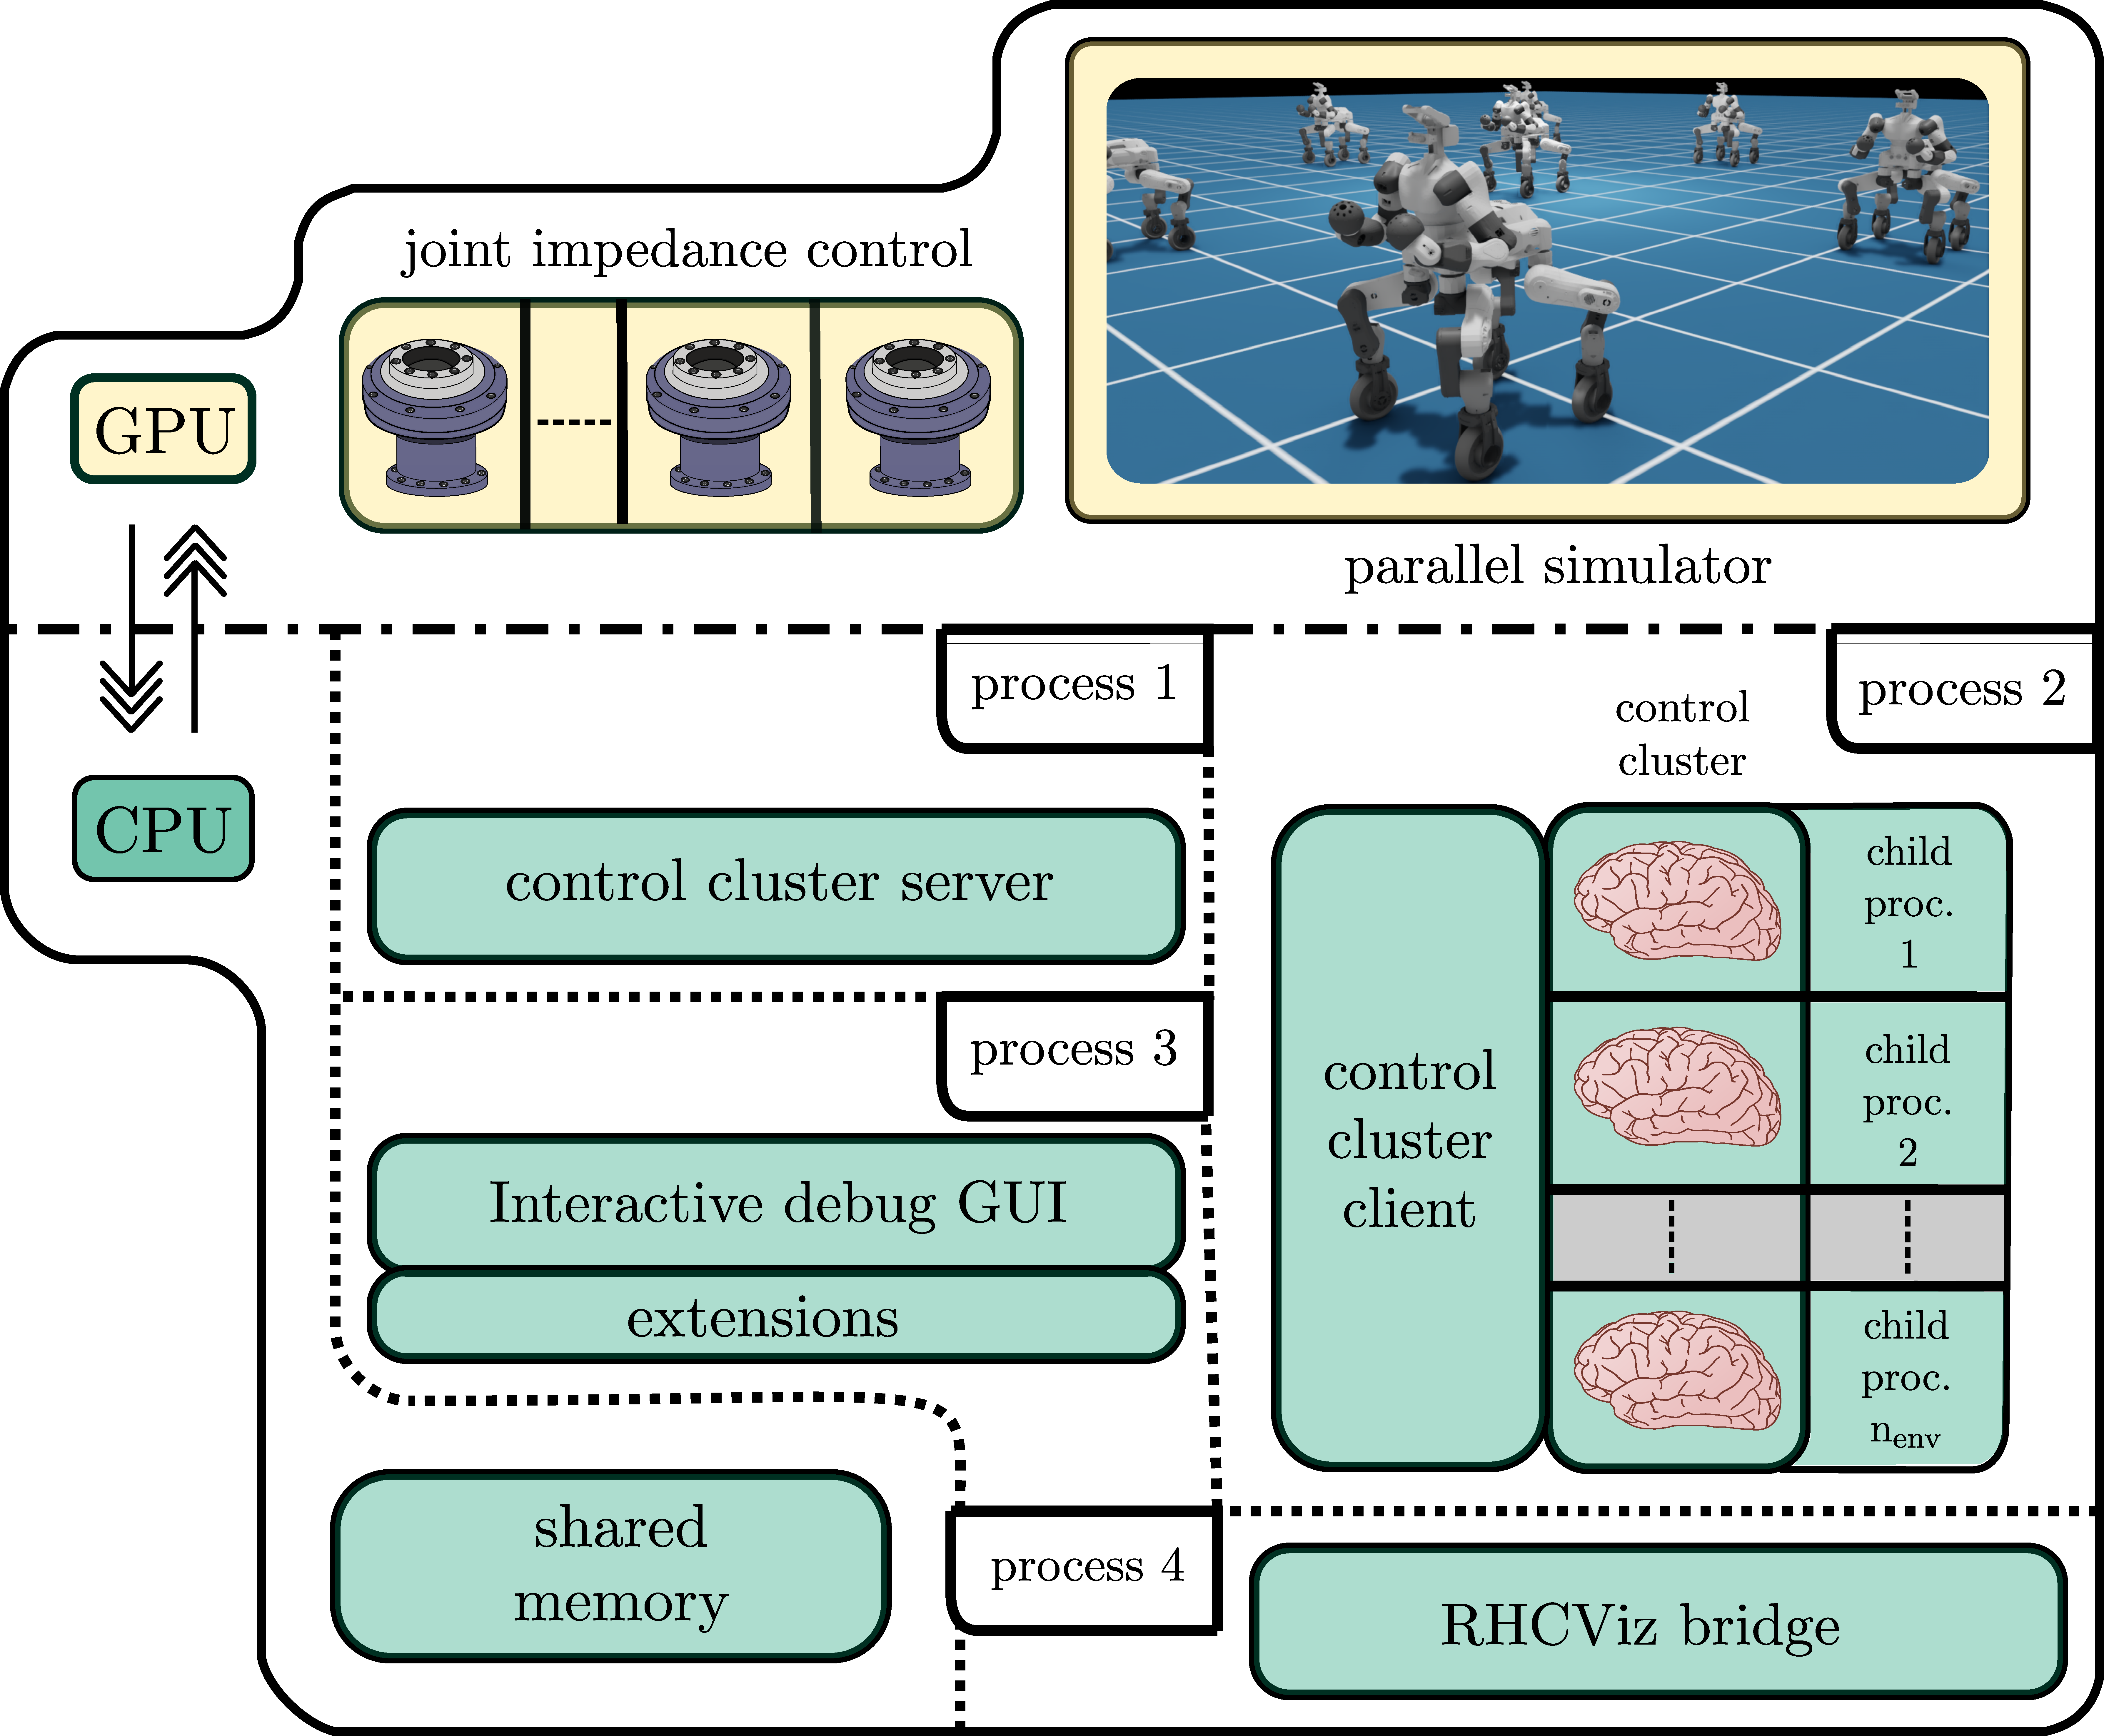
\includegraphics[width=0.9\columnwidth]{imgs/cocluster_arch.pdf}
	\caption{High-level overview of the software implementation of the training environment to which the agent is exposed: the robot in the simulator is controlled through a joint-level impedance controller, which is in turn used by a higher-level receding horizon controller. The agent can indirectly control the robot through the latter.}
	\label{fig:coclbridge_arch}
\end{figure}
\cite{rl:mujocoaccelereted2023}
\cite{frameworks:mittal2023orbit}

Fig.~\ref{fig:coclbridge_arch} shown a high level overview if the main moduli the echosystem is composed of. Specifically, it makes use of the following software packages:
\begin{itemize}
	\item Omniverse \textit{IsaacSim}~\cite{rl:makoviychuk2021isaac} is employed for performing the parallel GPU-accelerated simulation.
	\item \textit{Horizon}~\cite{frameworks::horizon_to} is employed for formulating the RHC controller, with an iLQR solver employed for computing the actual solution. Each controller is spawned in its own process using python's multiprocessing module.
	\item \textit{SharsorIPCpp}~\cite{mystuff::sharsoripcpp} is employed as a shared memory backend for fast data sharing between all the components on CPU.
	\item \textit{OmniRoboGym}~\cite{mystuff::omnirobogym} is used as a wrapper around IsaacSim and provides the \textit{simulation} environment.
	\item \textit{CoClusterBridge}~\cite{mystuff::coclusterbridge} is in charge of handling the connection and synchronization between the simulation environment and a cluster of RHC controllers. It furthermore provides an extensible debug GUI for monitoring the cluster and abstractions for the controllers.
	\item \textit{RHCViz}~\cite{mystuff::rhcviz} is a debug tool based on ROS1/ROS2 and RViz for visualizing RHC solutions in real-time. For our specific use case, it also allows to inspect a single environment during training without the need of any rendering on the simulator side.
	\item \textit{LRHControl}~\cite{mystuff::lrhccontrol} is the main package of the echosystem and is responsible for setting up the simulation environment, the control cluster, the (remote) training environment, the debug GUI (extensions included) and it currently utilizes a custom implementation of PPO~\cite{rl:schulman2017proximal} for training agents.
\end{itemize}





\section{A proof-of-concept example: \textnormal{\textit{learning acyclic stepping for locomotion}}}
\begin{figure}[t]
	\centering
	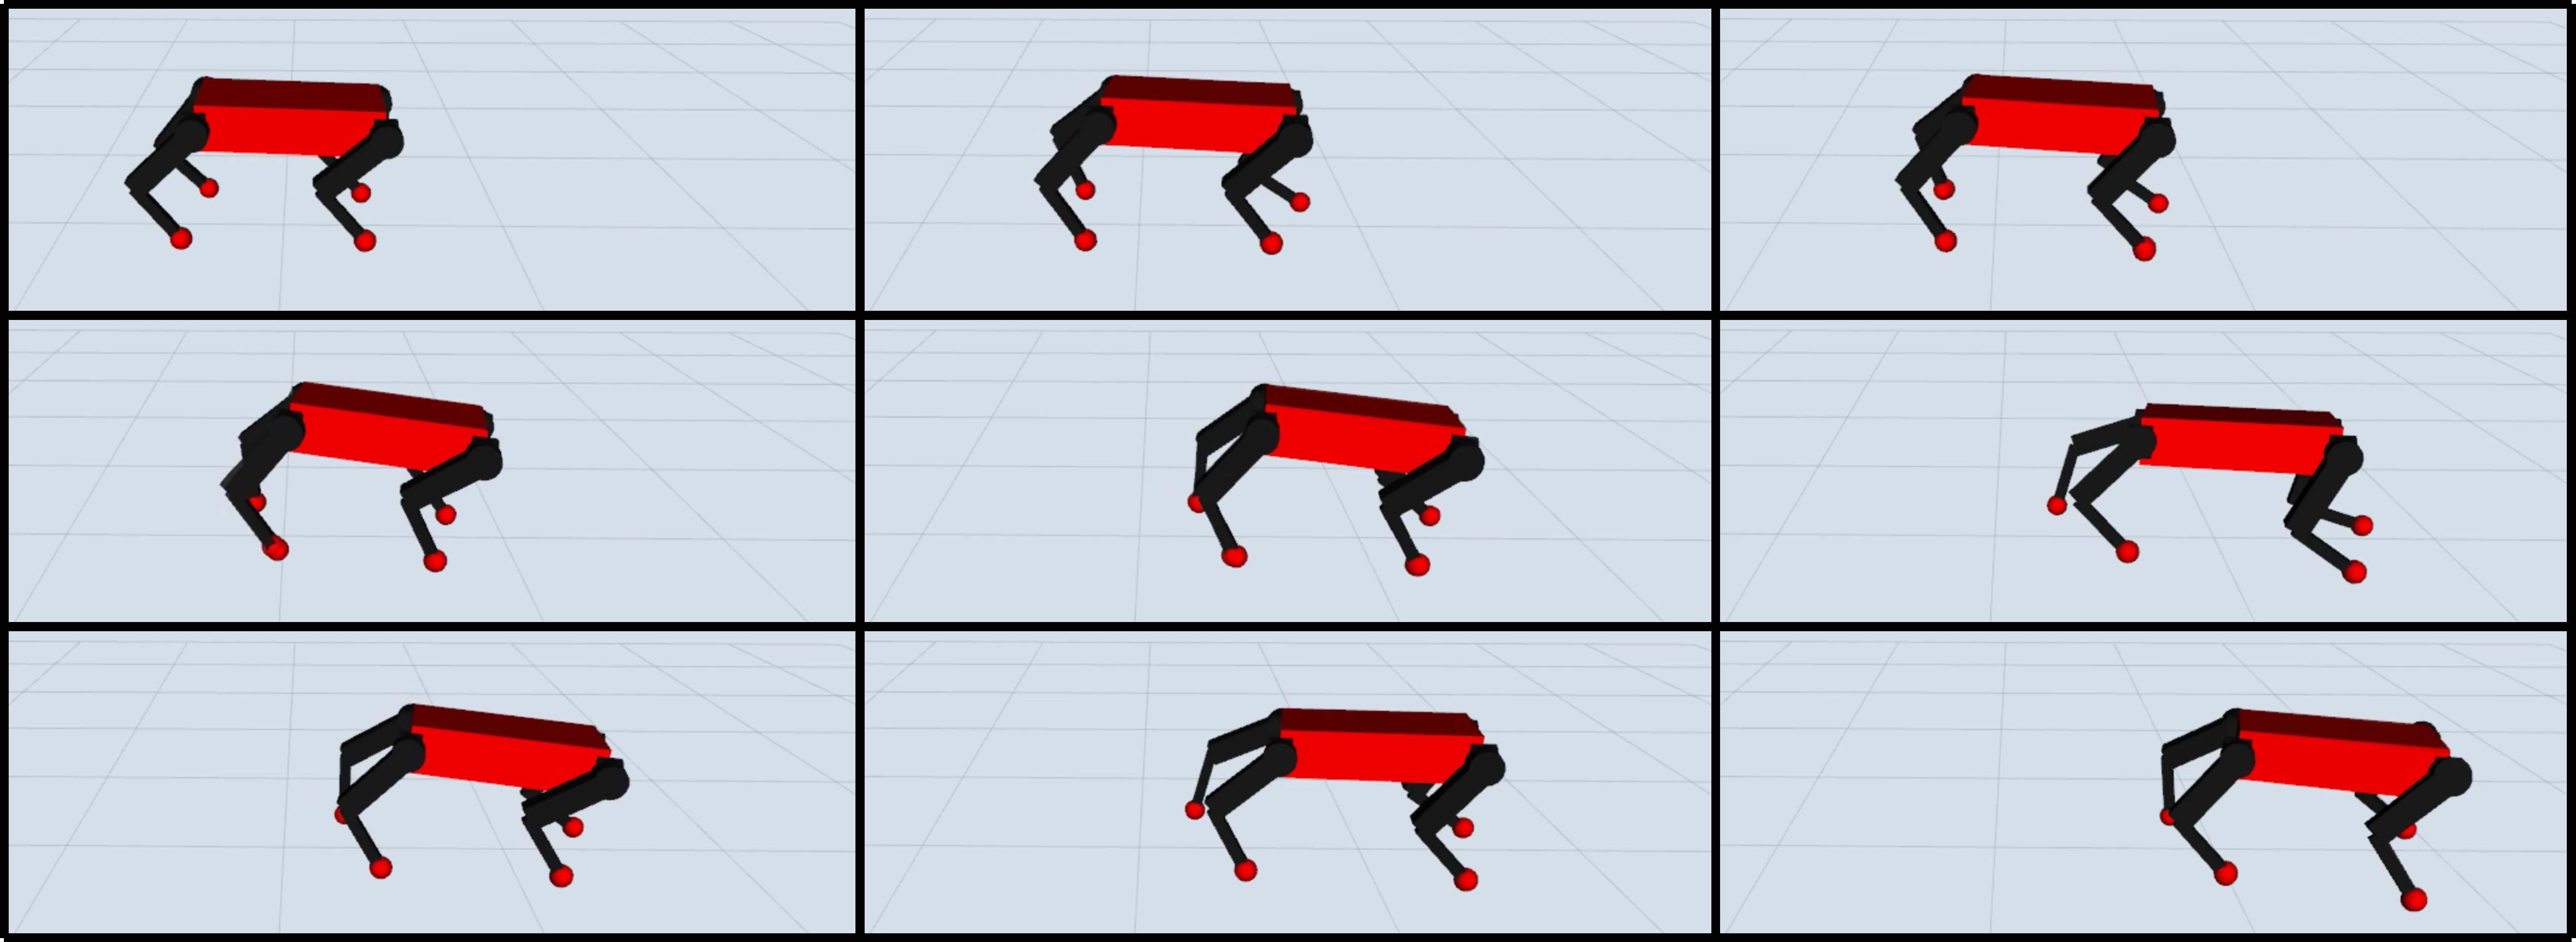
\includegraphics[width=0.9\columnwidth]{imgs/proof_of_concept.pdf}
	\caption{Preliminary results showing the agent during learning while it moves the robot forward using the RHC controller, from right to left and from top to bottom. The corresponding video is available at~\cite{web::poc_link}}
	\label{fig:proof}
\end{figure}
To showcase the potential of the proposed hybrid RL-RHC approach and of our framework, we trained a RL agent using PPO~\cite{rl:schulman2017proximal} to exploit a RHC controller for achieving a very simple forward locomotion task on a quadruped robot (shown in Fig.~\ref{fig:proof}). The agent is given a forward velocity reference to track and is continuously rewarded based on the task error and the performance of the underlying RHC controller. Notably, we observe the emergence of completely acyclic contact phases, varying from crawling to bound-like patterns.
 
\input{07-future_work}
\bibliographystyle{ieeetr}
\bibliography{bibliography/refs}

\end{document}
